\documentclass{beamer}

\setlength{\unitlength}{1cm} 
\usetheme{Singapore}

\usepackage[utf8]{inputenc}

\usepackage{amsmath}
\usepackage{graphicx}
\usepackage{tikz}
\usepackage[english]{babel}

\usepackage{apacite}
\bibliographystyle{apa}

% Graphs
\usetikzlibrary{positioning}
\tikzset{main node/.style={circle, draw,minimum size=1cm,inner sep=3pt},}


\newcommand{\mapsfrom}{\mathrel{\reflectbox{\ensuremath{\mapsto}}}}
\newcommand{\E}{\mathop{\mathbb{E}}}

\title{Can Central Bank operate under negative capital?}
\author{Andrea Titton}
\date{\today}

\begin{document}

\begin{frame}[plain]
    \titlepage
\end{frame}

\section{Introduction}

\begin{frame}{Motivation}
    \begin{columns}
        \begin{column}{.49\textwidth}
            \begin{itemize}
                \setlength\itemsep{1em}
                \item Times of uncertainty around the profitability of CBs
                \item Increased involvement of the CB in fiscal policy
                \item Fiscal dominance
            \end{itemize}
        \end{column}
        \begin{column}{.49\textwidth}
            \begin{figure}
                \includegraphics[width=\textwidth]{graphs/ecb-profits.PNG}
            \end{figure}
        \end{column}
    \end{columns}
\end{frame}

\begin{frame}{Points of view}
    \begin{itemize}
        \setlength\itemsep{1em}
        \item Historical perspective - emergence of the role of central banks, 19th century England and France
        \item The Central Bank as a fiscal agent
        \item Negative capital in an open economy at the ZLB
    \end{itemize}
\end{frame}

\section{Historical perspective - Flandreau}

\begin{frame}{Emergence of private Central Bank}
    Why do central banks have balance sheets?
    Evidence from the 19th century France and England. CB as...
    \vfill
    \begin{itemize}
        \setlength\itemsep{1em}
        \item a private (regulated) monopoly on liquidity supply
        \item alignment of private incentive and public interest
        \item high shareholders profits
    \end{itemize}
\end{frame}

\begin{frame}{Incentives of seigniorage maximizing government}
    Government that maximizes seigniorage has no incentive to react to real economy $r$. At $b\xrightarrow{} \infty$, cannot collect real resources
    \vfill
    \centering
    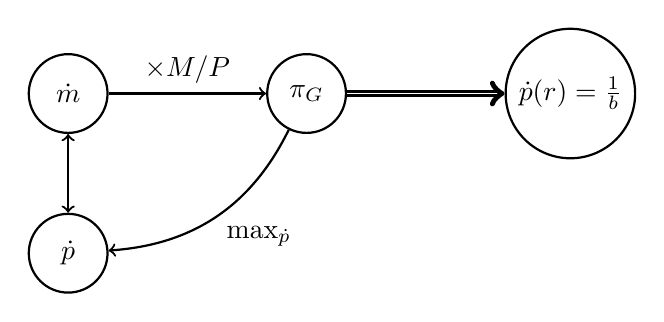
\begin{tikzpicture}[->, thick]
        % Nodes
        \node[main node] (1) {$\dot{m}$};
        \node[main node] [below = 1cm of 1] (2) {$\dot{p}$};
        \node[main node] [right = 2cm of 1] (3) {$\pi_G$};
        \node[main node] [right = 2cm of 3] (4) {$\dot{p}(r) = \frac{1}{b}$};
        % Paths
        \path[draw,thick]
        (1) edge [<->] node {} (2)
        (1) edge node [above] {$\times M / P$} (3)
        (3) edge [bend left] node [below right] {$\max_{\dot{p}}$} (2)
        (3) edge [double] node {} (4);
    \end{tikzpicture}
\end{frame}

\begin{frame}{Incentives of Private Central Bank}
    Profit maximizing Central Bank wants to maximize demand real money balances, which increases profit from lending. At $b\xrightarrow{} \infty$ converges to Friedman rule.
    \vfill
    \centering
    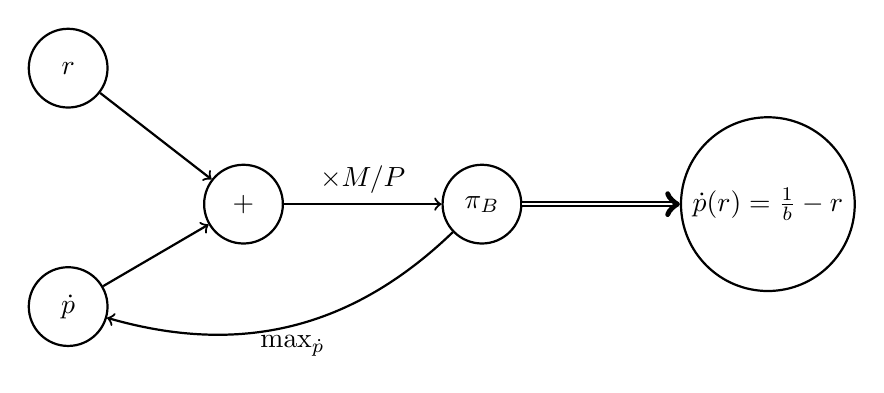
\begin{tikzpicture}[->, thick]
        % Nodes
        \node[main node] (1) {$r$};
        \node[main node] [below = 2cm of 1] (2) {$\dot{p}$};
        \node[main node] [below right = 1cm and 1.5cm of 1] (3) {$+$};
        \node[main node] [right = 2cm of 3] (4) {$\pi_B$};
        \node[main node] [right = 2cm of 4] (5) {$\dot{p}(r) = \frac{1}{b} -r$};
        % Paths
        \path[draw,thick]
        (1) edge node {} (3)
        (2) edge node {} (3)
        (3) edge node [above] {$\times M/P$} (4)
        (4) edge [bend left] node [below] {$\max_{\dot{p}}$} (2)
        (4) edge [double] node {} (5);
    \end{tikzpicture}
\end{frame}

\begin{frame}{Bagehot’s  rule, lender of last result}
    \begin{figure}
        \includegraphics[height=0.85\textheight]{graphs/bof-profit.PNG}
    \end{figure}
\end{frame}


\section{Central Bank solvency - Reis}

\begin{frame}{Central bank as fiscal agent - closed economy}
    \centering
    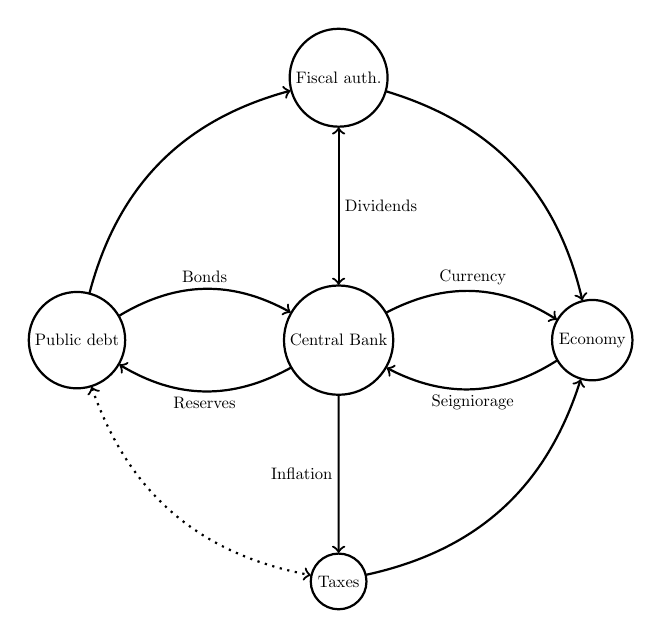
\begin{tikzpicture}[->, thick, scale=0.6, every node/.style={scale=0.6}]
        % Nodes
        \node[main node] (1) {Central Bank};
        \node[main node] [right = 2cm of 1] (2) {Economy};
        \node[main node] [below = 2cm of 1] (3) {Taxes};
        \node[main node] [left = 2cm of 1] (4) {Public debt};
        \node[main node] [above = 2cm of 1] (5) {Fiscal auth.};
        % Paths
        \path[draw,thick]
        (1) edge [bend left] node [above] {Currency} (2)
        (2) edge [bend left] node [below] {Seigniorage} (1)
        (1) edge node [left] {Inflation} (3)
        (1) edge [bend left] node [below] {Reserves} (4)
        (4) edge [bend left] node [above] {Bonds} (1)
        (1) edge [<->] node [right] {Dividends} (5)
        % Circular
        (5) edge [bend left] node {} (2)
        (3) edge [bend right] node {} (2)
        (4) edge [bend left] node {} (5)
        (4) edge [<->, dotted, bend right] node {} (3);
    \end{tikzpicture}
\end{frame}

\begin{frame}{Reserves flows, one period solvency}
    In a closed economy, given a current period solvency constraint, negative capital can be sustained either via \textit{seigniorage} or \textit{recapitalization} (i.e. $d_t < 0$).
    \begin{equation}
        v_t \mapsfrom (1 + r_t) \cdot v_{t-1} - \underbrace{(s_t)}_{seigniorage} + \overbrace{(d_t)}^{dividends} + \underbrace{q_t \cdot b_t - \delta_{t} \cdot b_{t-1}}_{\textit{public debt revenue}}
    \end{equation}
\end{frame}

\begin{frame}{Reserves flows, multiple period solvency}
    In a closed economy, negative capital can be sustained by deferring recapitalization using present value \textit{seigniorage}. Assuming $d_t = 0 \ \forall t$,
    \begin{equation*}
        \begin{split}
            \underbrace{\E\left(\sum_{j=0}^\infty m_{t, t+j} \cdot s_{t+j} \right)}_{\textit{present value seigniorage}} - \underbrace{(1 + r_t) \cdot v_t}_{\textit{current capital}} + \underbrace{\frac{\delta_t B_{t-1}}{p_t}}_{\textit{bond value}} \geq \\ \underbrace{\E\left(\sum_{j=0}^\infty m_{t, t+j} \cdot d_{t+j} \right)}_{\textit{present value dividends}}
        \end{split}
    \end{equation*}
\end{frame}

\section{Open economy - Farhi et al.}

\begin{frame}{A more contemporary approach}
    What about negative capital in an open economy? \vfill
    Negative capital can have effects on exchange rate (Beggar-thy-neighbor) and be seen as a fiscal expansion. \vfill
    Using framework by Caballero, Farhi, and Gourinchas (2016).
\end{frame}


% Bibliography
\nocite{*}

\begin{frame}[allowframebreaks]{References}
    \bibliography{refs}
\end{frame}

\end{document}